\documentclass[a4paper,11pt]{article}
\usepackage{amsmath,amsthm,amsfonts,amssymb,amscd,amstext,vmargin,graphics,graphicx,tabularx,multicol} \usepackage[french]{babel}
\usepackage[utf8]{inputenc}  
\usepackage[T1]{fontenc} 
\usepackage[T1]{fontenc}
\usepackage{amsmath,amssymb}
\usepackage{pstricks-add,tikz,tkz-tab,variations}
\usepackage[autolanguage,np]{numprint} 

\setmarginsrb{1.5cm}{0.5cm}{1cm}{0.5cm}{0cm}{0cm}{0cm}{0cm} %Gauche, haut, droite, haut
\newcounter{numexo}
\newcommand{\exo}[1]{\stepcounter{numexo}\noindent{\bf Exercice~\thenumexo} : \marginpar{\hfill /#1}}
\reversemarginpar


\newcounter{enumtabi}
\newcounter{enumtaba}
\newcommand{\q}{\stepcounter{enumtabi} \theenumtabi.  }
\newcommand{\qa}{\stepcounter{enumtaba} (\alph{enumtaba}) }
\newcommand{\initq}{\setcounter{enumtabi}{0}}
\newcommand{\initqa}{\setcounter{enumtaba}{0}}

\newcommand{\be}{\begin{enumerate}}
\newcommand{\ee}{\end{enumerate}}
\newcommand{\bi}{\begin{itemize}}
\newcommand{\ei}{\end{itemize}}
\newcommand{\bp}{\begin{pspicture*}}
\newcommand{\ep}{\end{pspicture*}}
\newcommand{\bt}{\begin{tabular}}
\newcommand{\et}{\end{tabular}}
\renewcommand{\tabularxcolumn}[1]{>{\centering}m{#1}} %(colonne m{} centrée, au lieu de p par défault) 
\newcommand{\tnl}{\tabularnewline}

\newcommand{\trait}{\noindent \rule{\linewidth}{0.2mm}}
\newcommand{\hs}[1]{\hspace{#1}}
\newcommand{\vs}[1]{\vspace{#1}}

\newcommand{\N}{\mathbb{N}}
\newcommand{\Z}{\mathbb{Z}}
\newcommand{\R}{\mathbb{R}}
\newcommand{\C}{\mathbb{C}}
\newcommand{\Dcal}{\mathcal{D}}
\newcommand{\Ccal}{\mathcal{C}}
\newcommand{\mc}{\mathcal}

\newcommand{\vect}[1]{\overrightarrow{#1}}
\newcommand{\ds}{\displaystyle}
\newcommand{\eq}{\quad \Leftrightarrow \quad}
\newcommand{\vecti}{\vec{\imath}}
\newcommand{\vectj}{\vec{\jmath}}
\newcommand{\Oij}{(O;\vec{\imath}, \vec{\jmath})}
\newcommand{\OIJ}{(O;I,J)}

\newcommand{\bmul}[1]{\begin{multicols}{#1}}
\newcommand{\emul}{\end{multicols}}


\newcommand{\reponse}[1][1]{%
\multido{}{#1}{\makebox[\linewidth]{\rule[0pt]{0pt}{20pt}\dotfill}
}}

\newcommand{\titre}[5] 
% #1: titre #2: haut gauche #3: bas gauche #4: haut droite #5: bas droite
{
\noindent #2 \hfill #4 \\
#3 \hfill #5

\vspace{-1.6cm}

\begin{center}\rule{6cm}{0.5mm}\end{center}
\vspace{0.2cm}
\begin{center}{\large{\textbf{#1}}}\end{center}
\begin{center}\rule{6cm}{0.5mm}\end{center}
}



\begin{document}
\pagestyle{empty}
\titre{Interrogation : Les probabilités}{Nom :}{Prénom :}{Classe}{Date}




\exo{2}
On lance un dé équilibré à 6 faces et on regarde le numéro sur la face supérieure. \\
Préciser la nature de chacun des événements suivants (événement élémentaire, impossible ou certain) :\\
A = « on obtient 2 » ;\\
B = « on obtient un chiffre pair » ;\\
C = « on obtient un nombre négatif » ;\\
D = « on obtient un chiffre strictement supérieur à 5 » ;\\
E = « on obtient un nombre entier ».\\
F= " on obtient un diviseur de 25".\\

\noindent \reponse[5]\\

\vspace*{0.5cm}

\exo{2} 

Pour gagner à ce jeu, il faut tomber sur la couleur rouge. On a le choix entre une roulette, un dé et une urne contenant dix boules.\\

\includegraphics[scale=0.9]{exoproba1.eps}\\ 
Que faut-il choisir pour avoir le plus de chance de gagner : la roulette, le dé ou l'urne ? (\textbf{Justifier votre réponse avec des probabilités.})\\
 \reponse[6]\\

\newpage

 \reponse[6]\\


\exo{2} 

On prend deux dés cubiques non truqués. On les lance et on ajoute les deux nombres obtenus.\\

\initq  \q Combien y a-t-il d'issues possibles ? Citer-les.\\
\reponse[4]\\

\q Quelle est la probabilité d'obtenir 9 ?\\
\reponse[8]\\

\exo{4} On propose le jeu suivant : le joueur fait tourner la roue puis tire une boule dans l'urne.\\
Si la couleur du secteur de la roue et la bille sont vertes, le joueur gagne une casquette.\\
Si la couleur du secteur de la roue et la bille sont rouges, le joueur gagne une écharpe.\\
Si le joueur obtient du vert et du rouge (peu importe si c'est le secteur ou la boule) alors le joueur gagne un maillot dédicacé par les joueurs du club.\\

\includegraphics[scale=0.75]{exoproba2.eps} \\

\newpage

\initq  \q Construire l'arbre \textbf{pondéré} de l'expérience aléatoire ci-dessus.\\

\vspace*{10cm}

\q Quelle est la probabilité de gagner une casquette ? Justifier avec un calcul.\\
\reponse[6]\\

\q Quelle est la probabilité de gagner un maillot dédicacé ?  Justifier avec un calcul.\\
\reponse[6]\\




\end{document}
